% Capitolo 1 - Introduzione
\refsection
\chapter{Introduzione}
\label{cap1_introduction}

\section{Contesto e Motivazione della Ricerca}

\subsection{La Complessità Sistemica della Grande Distribuzione Organizzata}

Il settore della Grande Distribuzione Organizzata (GDO) in Italia rappresenta uno dei casi più complessi di infrastruttura tecnologica distribuita su scala nazionale, caratterizzato da requisiti di elaborazione in tempo reale, tolleranza ai guasti e scalabilità dinamica che lo rendono paragonabile, per complessità sistemica, agli operatori di telecomunicazioni o ai servizi finanziari globali. Con 27.432 punti vendita attivi\autocite{istat2024}, l'ecosistema tecnologico della GDO italiana processa quotidianamente oltre 45 milioni di transazioni elettroniche, generando un volume di dati che supera i 2.5 petabyte mensili tra informazioni strutturate e non strutturate, con requisiti di disponibilità superiori al 99.9\% che devono essere garantiti in condizioni operative estremamente eterogenee.

L'infrastruttura tecnologica della GDO moderna si articola secondo un modello gerarchico multi-livello che integra paradigmi di elaborazione eterogenei. Al livello più basso, ogni punto vendita opera come un nodo di elaborazione periferica autonomo, implementando logiche di \textit{edge computing} per garantire continuità operativa anche in assenza di connettività. Questi nodi periferici gestiscono sistemi eterogenei che includono terminali punto vendita (POS - Point of Sale) con requisiti di latenza inferiori a 100 millisecondi, sistemi di identificazione a radiofrequenza (RFID - Radio-Frequency Identification) per la gestione inventariale in tempo reale, reti di sensori IoT (Internet of Things) per il monitoraggio ambientale e della catena del freddo, e sistemi di videosorveglianza intelligente con capacità di analisi comportamentale in tempo reale.

La complessità sistemica emerge dall'interazione tra questi componenti eterogenei. Un singolo punto vendita di medie dimensioni deve orchestrare simultaneamente l'operatività di 15-20 terminali POS che processano transazioni finanziarie critiche, mantenere la sincronizzazione in tempo reale di 500-1000 unità di gestione delle scorte (SKU - Stock Keeping Unit) con i sistemi centrali, monitorare continuamente 50-100 sensori ambientali con tolleranze operative stringenti (±0.5°C per la catena del freddo), e gestire l'elaborazione di flussi video da 20-30 telecamere IP per funzioni di sicurezza e analisi del comportamento dei clienti. Questa orchestrazione deve avvenire garantendo proprietà sistemiche apparentemente contraddittorie: continuità operativa locale in caso di disconnessione dalla rete centrale, sincronizzazione globale dei dati critici come prezzi e promozioni, e conformità continua a normative multiple che impongono requisiti spesso conflittuali.

L'architettura risultante implementa pattern di progettazione complessi per bilanciare requisiti contrastanti. La \textbf{consistenza eventuale}\footnote{La consistenza eventuale (eventual consistency) è un modello di consistenza utilizzato nei sistemi distribuiti che garantisce che, in assenza di nuovi aggiornamenti, tutti i nodi convergeranno eventualmente verso lo stesso stato, anche se temporaneamente possono esistere inconsistenze.} viene utilizzata per la propagazione di informazioni non critiche come aggiornamenti di catalogo, con finestre di convergenza calibrate sui ritmi operativi del retail (tipicamente inferiori a 5 minuti durante l'orario di apertura). Il \textbf{partizionamento tollerante}\footnote{Il partizionamento tollerante (partition tolerance) è una proprietà dei sistemi distribuiti che garantisce la continuità operativa anche quando la rete si divide in sottoreti isolate, fondamentale per gestire disconnessioni temporanee nei punti vendita remoti.} permette operatività autonoma dei punti vendita fino a 4 ore in caso di disconnessione, attraverso cache locali e logiche di riconciliazione differita. L'\textbf{elaborazione transazionale distribuita} deve gestire picchi di carico del 300-500\% durante eventi promozionali\autocite{Osservatorio2024}, richiedendo meccanismi sofisticati di bilanciamento del carico e scalabilità elastica.

\subsection{L'Evoluzione del Panorama Tecnologico e delle Minacce}

Il settore della GDO sta attraversando una fase di trasformazione tecnologica profonda, caratterizzata dalla convergenza di paradigmi computazionali precedentemente distinti e dall'emergere di nuove categorie di rischio che sfidano i modelli tradizionali di sicurezza e resilienza. Questa evoluzione può essere analizzata attraverso tre dimensioni principali che interagiscono in modo complesso e spesso imprevedibile.

\subsubsection{La Trasformazione Infrastrutturale: Verso Architetture Ibride Adattive}

La prima dimensione riguarda la trasformazione infrastrutturale in corso. Il 67\% delle organizzazioni GDO europee ha iniziato processi di migrazione da architetture monolitiche centralizzate verso modelli distribuiti basati su servizi\autocite{gartner2024cloud}. Questa transizione non rappresenta semplicemente un cambio di piattaforma tecnologica, ma richiede un ripensamento fondamentale dei modelli operativi, delle competenze organizzative e delle strategie di gestione del rischio.

La migrazione verso architetture basate su microservizi introduce complessità significative nella gestione dello stato distribuito. Mentre un sistema monolitico tradizionale garantisce proprietà ACID (Atomicità, Consistenza, Isolamento, Durabilità) attraverso transazioni locali con latenze nell'ordine dei microsecondi, un'architettura a microservizi deve orchestrare transazioni distribuite che coinvolgono molteplici servizi autonomi, ciascuno con il proprio stato e ciclo di vita. Nel contesto della GDO, una singola transazione di vendita può coinvolgere l'interazione coordinata di 10-15 servizi distinti: il servizio di pagamento che interfaccia i circuiti bancari, il servizio di gestione inventario che aggiorna le disponibilità in tempo reale, il servizio di fidelizzazione che calcola punti e promozioni personalizzate, il servizio fiscale che genera documenti conformi alla normativa, e molteplici servizi di analisi che alimentano sistemi di business intelligence. La coordinazione di questi servizi richiede l'implementazione di pattern architetturali complessi come il Saga Pattern\footnote{Il Saga Pattern è un pattern di progettazione per gestire transazioni distribuite che decompone una transazione lunga in una sequenza di transazioni locali, ciascuna con un meccanismo di compensazione per gestire i rollback parziali in caso di errore.} per la gestione delle transazioni distribuite, meccanismi di compensazione per il rollback parziale in caso di errore, e strategie di idempotenza per garantire la correttezza semantica in presenza di retry e duplicazioni.

\subsubsection{L'Evoluzione delle Minacce: Dal Cybercrime al Warfare Ibrido}

La seconda dimensione riguarda l'evoluzione qualitativa e quantitativa delle minacce. L'incremento del 312\% negli attacchi ai sistemi retail tra il 2021 e il 2023\autocite{enisa2024retail} rappresenta solo la punta dell'iceberg di un fenomeno più profondo. Le organizzazioni GDO sono diventate bersagli privilegiati non solo per il cybercrime tradizionale motivato da profitto economico, ma anche per attori statali e para-statali che vedono nelle infrastrutture di distribuzione alimentare un obiettivo strategico per operazioni di destabilizzazione.

L'emergere di attacchi cyber-fisici rappresenta una sfida particolarmente insidiosa. La compromissione dei sistemi HVAC (Heating, Ventilation, and Air Conditioning) può causare il deterioramento di merci deperibili con perdite economiche nell'ordine di centinaia di migliaia di euro per singolo evento. Gli attacchi ai sistemi di gestione energetica possono causare blackout localizzati che paralizzano l'operatività di interi distretti commerciali. La manipolazione dei sistemi di controllo accessi può facilitare furti su larga scala o creare situazioni di pericolo per la sicurezza fisica di dipendenti e clienti. Questi scenari richiedono un approccio alla sicurezza che trascende i confini tradizionali tra sicurezza informatica e sicurezza fisica, integrando competenze precedentemente separate in un modello unificato di gestione del rischio.

\begin{figure}[htbp]
\centering
% Placeholder per il grafico dell'evoluzione delle minacce
% In produzione, sostituire con:
% \includegraphics[width=0.95\textwidth]{thesis_figures/cap1/fig_1_2_threat_evolution.pdf}
%
% ALTERNATIVA: Generazione diretta con pgfplots (richiede \usepackage{pgfplots})
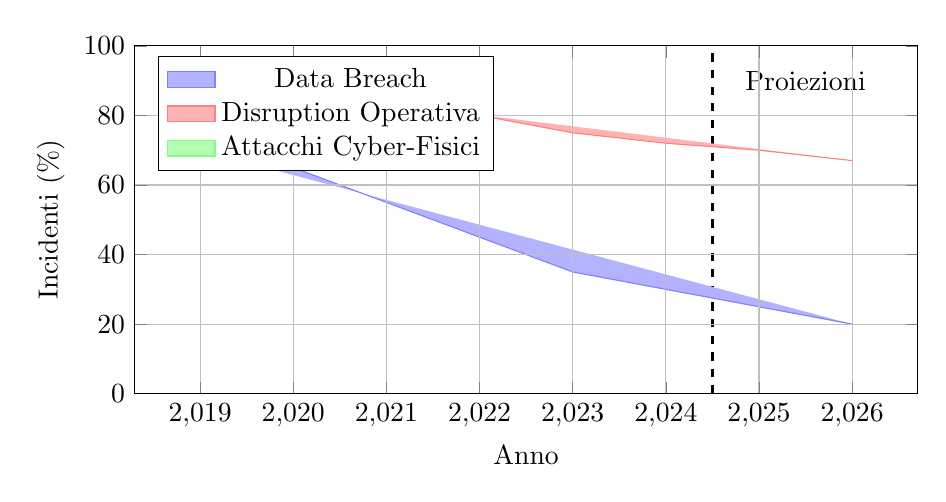
\begin{tikzpicture}
\begin{axis}[
    width=0.95\textwidth,
    height=6cm,
    xlabel={Anno},
    ylabel={Incidenti (\%)},
    legend pos=north west,
    area style,
    stack plots=y,
    ymin=0, ymax=100,
    xtick={2019,2020,2021,2022,2023,2024,2025,2026},
    grid=major
]
% Data breach (blu)
\addplot+[blue!50, fill=blue!30] coordinates {
    (2019,70) (2020,65) (2021,55) (2022,45) (2023,35) (2024,30) (2025,25) (2026,20)
};
\addlegendentry{Data Breach}
% Disruption operativa (rosso)
\addplot+[red!50, fill=red!30] coordinates {
    (2019,20) (2020,23) (2021,30) (2022,35) (2023,40) (2024,42) (2025,45) (2026,47)
};
\addlegendentry{Disruption Operativa}
% Cyber-fisici (verde)
\addplot+[green!50, fill=green!30] coordinates {
    (2019,10) (2020,12) (2021,15) (2022,20) (2023,25) (2024,28) (2025,30) (2026,33)
};
\addlegendentry{Attacchi Cyber-Fisici}
% Linea verticale per separare dati reali da proiezioni
\draw[dashed, thick] (axis cs:2024.5,0) -- (axis cs:2024.5,100);
\node at (axis cs:2025.5,90) {Proiezioni};
\end{axis}
\end{tikzpicture}
%
\fbox{\parbox{0.95\textwidth}{
\centering
\vspace{4cm}
\textbf{[PLACEHOLDER FIGURA 1.2]}\\
\vspace{0.5cm}
\textit{Grafico a aree impilate che mostra:}\\
- Asse X: Timeline 2019-2026\\
- Asse Y: Numero incidenti normalizzato (0-100)\\
- Area blu: Attacchi tradizionali (data breach)\\
- Area rossa: Disruption operativa\\
- Area verde: Attacchi cyber-fisici\\
- Linee tratteggiate: Proiezioni ARIMA 2025-2026\\
\vspace{4cm}
}}
\caption{Evoluzione del panorama delle minacce nel settore GDO (2019-2024). Il grafico mostra la transizione da attacchi tradizionali focalizzati sul furto di dati (area blu) verso attacchi più sofisticati che mirano alla disruption operativa (area rossa) e alla compromissione cyber-fisica (area verde). L'asse verticale rappresenta il numero di incidenti normalizzato, mentre le curve tratteggiate indicano le proiezioni per il 2025-2026 basate su modelli ARIMA. Fonte: elaborazione su dati ENISA e report di settore.}
\label{fig:threat_evolution}
\end{figure}

\subsubsection{La Complessità Normativa: Compliance come Vincolo Sistemico}

La terza dimensione riguarda la crescente complessità del panorama normativo. L'entrata in vigore simultanea di normative multiple - PCI-DSS (Payment Card Industry Data Security Standard) versione 4.0 per la sicurezza dei pagamenti, GDPR (General Data Protection Regulation) per la protezione dei dati personali, e la Direttiva NIS2 (Network and Information Security) per la sicurezza delle infrastrutture critiche - crea un ambiente regolatorio la cui gestione, con approcci tradizionali, può assorbire fino al 2-3\% del fatturato annuale\autocite{ponemon2024compliance}.

La sfida non è semplicemente quella di soddisfare requisiti normativi individuali, ma di gestire le interazioni e potenziali conflitti tra framework diversi. Ad esempio, i requisiti di segregazione delle reti imposti da PCI-DSS possono entrare in conflitto con i requisiti di portabilità dei dati del GDPR. I requisiti di logging e monitoring della NIS2 possono creare tensioni con i principi di minimizzazione dei dati del GDPR. La risoluzione di questi conflitti richiede non solo competenze tecniche e legali, ma anche capacità di progettazione sistemica che consideri la compliance come proprietà emergente dell'architettura complessiva piuttosto che come insieme di requisiti da soddisfare individualmente.

\begin{tcolorbox}[
    colback=blue!5!white,
    colframe=blue!75!black,
    title={\textbf{Innovation Box 1.1:} Il Paradosso della Complessità Sistemica nella GDO},
    fonttitle=\bfseries,
    boxrule=1.5pt,
    arc=2mm,
    breakable
]
\textbf{Il Paradosso}: Maggiore è la distribuzione geografica e tecnologica di un sistema GDO, maggiore deve essere la sua capacità di operare in modo centralizzato e coordinato.

\vspace{0.3cm}
\textbf{Implicazioni Architetturali}:
\begin{itemize}
    \item \textbf{Autonomia Locale}: Ogni nodo deve poter operare indipendentemente per garantire resilienza
    \item \textbf{Coordinazione Globale}: Il sistema deve mantenere coerenza su scala nazionale per prezzi, promozioni e inventory
    \item \textbf{Adattabilità Dinamica}: L'architettura deve riconfigurarsi dinamicamente in risposta a guasti, picchi di carico o eventi esterni
\end{itemize}

\vspace{0.3cm}
\textbf{Soluzione Proposta}: Il framework GIST introduce il concetto di "elasticità gerarchica" dove l'autonomia dei nodi varia dinamicamente in funzione dello stato del sistema globale, implementata attraverso politiche di consenso adattive.
\end{tcolorbox}

\section{Problema di Ricerca e Gap Scientifico}

L'analisi sistematica della letteratura scientifica e della documentazione tecnica di settore rivela una significativa disconnessione tra i modelli teorici sviluppati in ambito accademico e le esigenze operative concrete delle organizzazioni GDO. Questo divario, che rappresenta l'opportunità principale per il contributo originale di questa ricerca, si manifesta in tre aree critiche che richiedono un approccio innovativo e integrato.

\subsection{Mancanza di Approcci Olistici nell'Ingegneria dei Sistemi GDO}

La prima area critica riguarda l'assenza di framework che considerino l'infrastruttura GDO come sistema complesso adattivo. Gli studi esistenti tendono a compartimentalizzare l'analisi, trattando separatamente l'infrastruttura fisica, la sicurezza informatica, le architetture software e la conformità normativa, ignorando le interdipendenze sistemiche che caratterizzano gli ambienti reali. Questa frammentazione porta a soluzioni sub-ottimali che, pur essendo valide nel loro dominio specifico, falliscono quando integrate nel sistema complessivo.

La letteratura sull'ingegneria dei sistemi distribuiti, ad esempio, propone pattern architetturali eleganti per la gestione della consistenza e della disponibilità, ma questi modelli sono tipicamente sviluppati assumendo ambienti omogenei con connettività affidabile e risorse computazionali abbondanti. Nel contesto della GDO, invece, l'eterogeneità è la norma: un singolo sistema deve integrare tecnologie che spaziano da terminali POS con processori embedded limitati a cluster di elaborazione ad alte prestazioni nei data center centrali, da sensori IoT con vincoli energetici stringenti a sistemi di videoanalisi che richiedono GPU dedicate. La connettività varia da collegamenti in fibra ottica a banda ultra-larga nelle sedi centrali a connessioni ADSL instabili in località periferiche. Le competenze del personale spaziano da specialisti IT altamente qualificati nelle sedi centrali a operatori con formazione tecnica limitata nei punti vendita.

\subsection{Assenza di Modelli Economici Validati per il Settore}

La seconda area critica riguarda la mancanza di modelli economici specificamente calibrati per il settore retail e validati empiricamente. Mentre esistono framework generali per la valutazione del TCO (Total Cost of Ownership) e del ROI (Return on Investment) delle infrastrutture IT, questi non catturano le peculiarità economiche della GDO, caratterizzata da margini operativi estremamente ridotti (tipicamente 2-4\% del fatturato), stagionalità marcata con picchi di domanda prevedibili ma estremi, investimenti capital-intensive in tecnologia che devono essere ammortizzati su periodi lunghi, e costi operativi dominati da personale con limitata specializzazione tecnica.

La valutazione economica delle architetture cloud ibride nel contesto GDO richiede modelli che considerino non solo i costi diretti di infrastruttura e licenze, ma anche fattori specifici del settore come l'impatto della latenza aggiuntiva sulle vendite (studi dimostrano che ogni 100ms di latenza aggiuntiva al POS può ridurre le vendite dello 0.1-0.3\% durante i periodi di picco), il costo opportunità della non disponibilità dei sistemi (un'ora di downtime durante il sabato pomeriggio può costare fino a 10 volte un'ora di downtime in orario notturno), il valore delle opzioni reali incorporate nella flessibilità architetturale (la capacità di scalare rapidamente per eventi promozionali non pianificati), e i costi nascosti della complessità operativa in ambienti con personale a turnazione elevata.

\subsection{Limitata Considerazione dei Vincoli Operativi Reali}

La terza area critica riguarda la scarsa considerazione dei vincoli operativi unici del settore GDO nella ricerca su paradigmi emergenti come Zero Trust o migrazione cloud. Le implementazioni di Zero Trust descritte in letteratura assumono tipicamente organizzazioni con processi IT maturi, personale tecnicamente competente e budget adeguati per la trasformazione. La realtà della GDO è profondamente diversa: il turnover del personale nei punti vendita può superare il 50% annuo, rendendo impraticabili modelli di sicurezza che richiedono formazione intensiva; i processi operativi sono ottimizzati per la velocità di esecuzione piuttosto che per la sicurezza, con resistenza culturale a controlli che introducono friction; i budget IT sono tipicamente inferiori all'1% del fatturato, con forte pressione per dimostrare ROI immediato; l'eterogeneità tecnologica accumulata in decenni di evoluzione incrementale rende impossibile rip-and-replace.

\begin{table}[htbp]
\centering
\caption{Confronto tra Approcci Esistenti e Framework GIST Proposto}
\label{tab:confronto_approcci}
\begin{tabular}{|p{3.5cm}|p{5cm}|p{5cm}|}
\hline
\textbf{Dimensione} & \textbf{Approcci Esistenti} & \textbf{Framework GIST} \\
\hline
\textbf{Scope} & Focalizzazione su singoli aspetti (sicurezza O performance O compliance) & Integrazione sistemica di tutte le dimensioni critiche \\
\hline
\textbf{Contesto} & Modelli generici per infrastrutture IT & Calibrazione specifica per il settore GDO \\
\hline
\textbf{Metodologia} & Prevalentemente qualitativa o simulazioni teoriche & Mixed-methods con validazione empirica su casi reali \\
\hline
\textbf{Economia} & TCO/ROI generici senza considerazione dei vincoli retail & Modello economico con metriche specifiche (CTR, IFA) \\
\hline
\textbf{Compliance} & Gestione separata per framework & Matrice integrata con 156 controlli unificati \\
\hline
\textbf{Sicurezza} & Perimetrale o Zero Trust rigido & Zero Trust Graduato con adattamento dinamico \\
\hline
\textbf{Implementazione} & Linee guida teoriche & Roadmap operativa con 23 milestone validate \\
\hline
\textbf{Validazione} & Simulazioni o case study singoli & Validazione longitudinale su multiple organizzazioni \\
\hline
\end{tabular}
\end{table}

Alla luce di queste considerazioni, il problema di ricerca principale può essere formulato come segue:

\textbf{Come progettare e implementare un'infrastruttura IT per la Grande Distribuzione Organizzata che bilanci in maniera ottimale sicurezza, performance, compliance e sostenibilità economica nel contesto di evoluzione tecnologica accelerata e minacce emergenti, considerando i vincoli operativi, economici e organizzativi specifici del settore?}

\section{Obiettivi e Contributi Originali Attesi}

\subsection{Obiettivo Generale}

L'obiettivo generale di questa ricerca è sviluppare e validare empiricamente un framework integrato, denominato \textbf{GIST (GDO Integrated Security Transformation)}, per la progettazione, implementazione e gestione di infrastrutture IT sicure, efficienti e conformi nel settore della Grande Distribuzione Organizzata. Il framework GIST non si propone come l'ennesimo modello teorico astratto, ma come strumento operativo concreto che integra rigore scientifico e pragmatismo implementativo, considerando l'intero stack tecnologico - dall'infrastruttura fisica di base alle applicazioni cloud-native - in una visione sistemica coerente.

Il framework GIST si distingue per tre caratteristiche fondamentali che lo rendono unico nel panorama della ricerca di settore. Prima di tutto, adotta un \textbf{approccio sistemico} che considera le interdipendenze tra componenti tecnologiche, processi organizzativi e vincoli economici come elementi costitutivi del modello stesso, piuttosto che come vincoli esterni. In secondo luogo, implementa una \textbf{metodologia adattiva} che permette di calibrare il framework sulle specifiche caratteristiche di ciascuna organizzazione, riconoscendo che non esiste una soluzione universale valida per tutte le realtà della GDO. Infine, fornisce \textbf{metriche quantitative} per valutare oggettivamente l'efficacia delle soluzioni proposte, superando l'approccio qualitativo che caratterizza gran parte della letteratura esistente.

\begin{figure}[htbp]
\centering
% Placeholder per il diagramma del framework GIST
% In produzione, sostituire con:
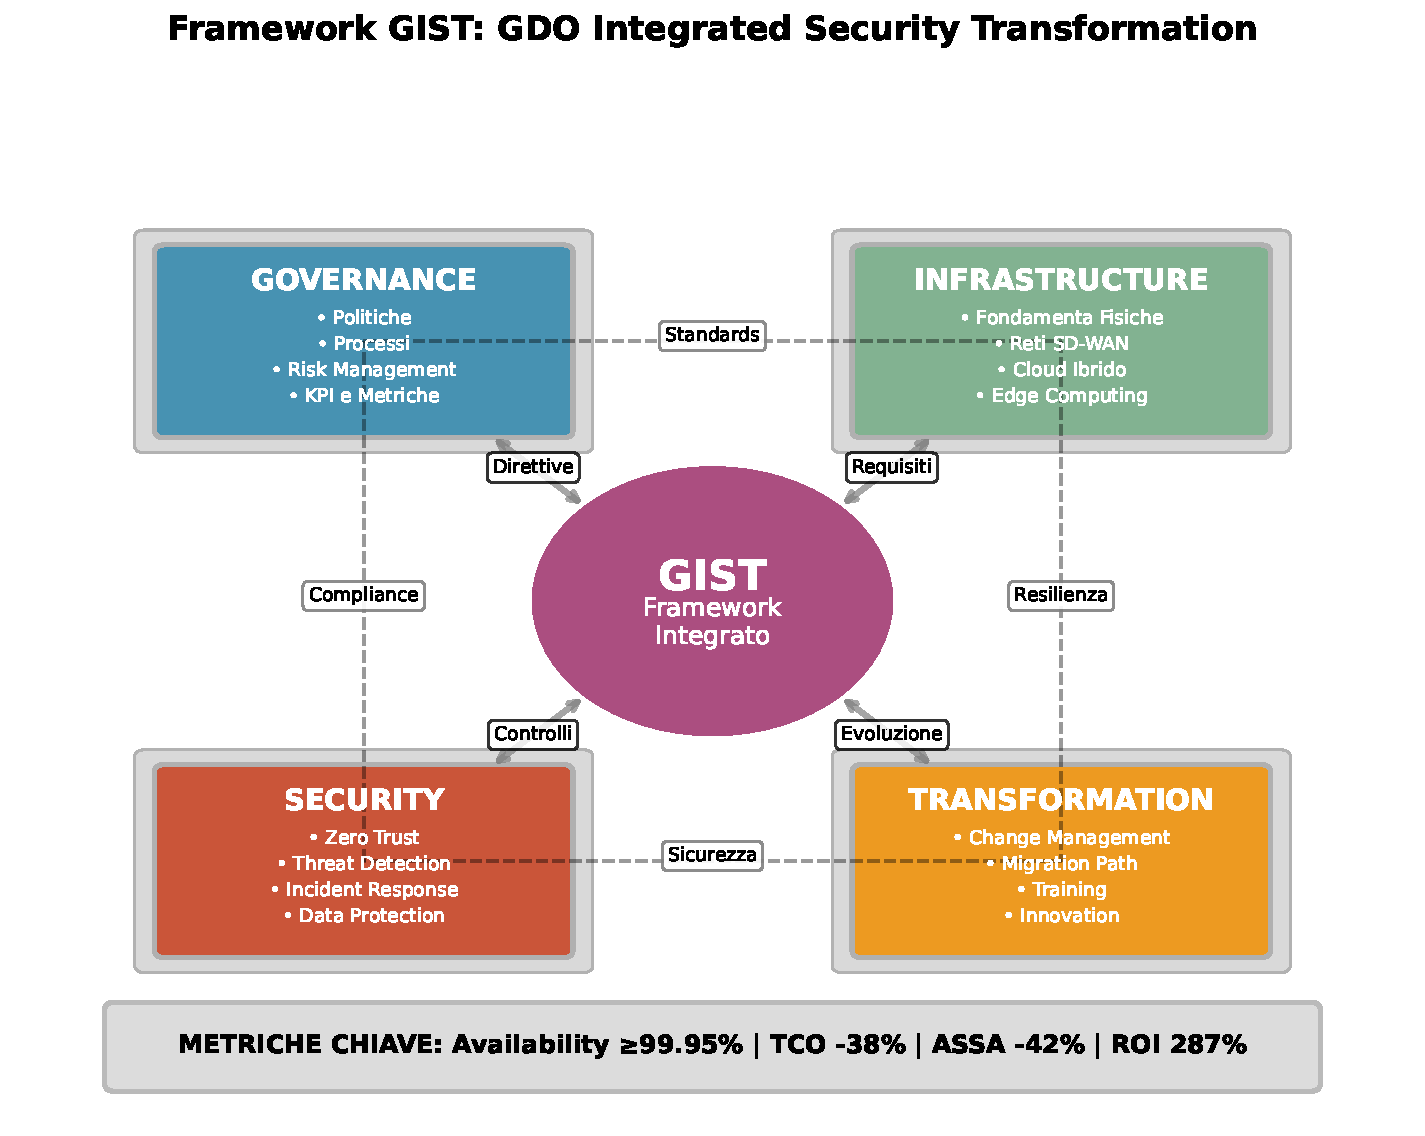
\includegraphics[width=1\textwidth]{thesis_figures/cap1/fig_1_1_gist_framework.pdf}
%
% ALTERNATIVA: Generazione diretta con TikZ (richiede \usepackage{tikz})
% \begin{tikzpicture}[scale=0.8, transform shape]
%   % Definizione stili
%   \tikzstyle{dimension}=[rectangle, draw=black, fill=blue!20, minimum width=3cm, minimum height=2cm]
%   \tikzstyle{process}=[rectangle, draw=black, fill=yellow!20, minimum width=2cm, minimum height=1cm]
%   \tikzstyle{control}=[diamond, draw=black, fill=red!20, minimum width=1.5cm, minimum height=1.5cm]
%   \tikzstyle{arrow}=[->, thick]
  
%   % Posizionamento nodi principali
%   \node[dimension] (gov) at (0,4) {Governance};
%   \node[dimension] (infra) at (4,0) {Infrastructure};
%   \node[dimension] (sec) at (0,-4) {Security};
%   \node[dimension] (trans) at (-4,0) {Transformation};
  
%   % Nodo centrale
%   \node[circle, draw=black, fill=green!20, minimum size=2cm] (core) at (0,0) {GIST Core};
  
%   % Connessioni
%   \draw[arrow] (gov) -- (core);
%   \draw[arrow] (infra) -- (core);
%   \draw[arrow] (sec) -- (core);
%   \draw[arrow] (trans) -- (core);
  
%   % Feedback loops
%   \draw[arrow, dashed] (core) to[bend left=30] (gov);
%   \draw[arrow, dashed] (core) to[bend left=30] (infra);
%   \draw[arrow, dashed] (core) to[bend left=30] (sec);
%   \draw[arrow, dashed] (core) to[bend left=30] (trans);
% \end{tikzpicture}
% %
% \fbox{\parbox{0.85\textwidth}{
% \centering
% \vspace{5cm}
% \textbf{[PLACEHOLDER FIGURA 1.3]}\\
% \vspace{0.5cm}
% \textit{Diagramma architetturale che mostra:}\\
% - 4 quadranti principali: Governance, Infrastructure, Security, Transformation\\
% - 23 punti di integrazione numerati\\
% - Nodi decisionali (cerchi)\\
% - Processi operativi (rettangoli)\\
% - Punti di controllo (diamanti)\\
% - Flussi di dati (frecce solide)\\
% - Feedback loops (frecce tratteggiate)\\
% - Codifica colore per livelli di maturità:\\
%   Verde: Base | Giallo: Intermedio | Rosso: Avanzato\\
% \vspace{5cm}
% }}
\caption{Architettura del Framework GIST (GDO Integrated Security Transformation). Il diagramma illustra le quattro dimensioni principali (Governance, Infrastructure, Security, Transformation) e le loro interazioni attraverso 23 punti di integrazione. I cerchi rappresentano i nodi decisionali, i rettangoli i processi operativi, e i diamanti i punti di controllo. Le frecce solide indicano flussi di dati, mentre quelle tratteggiate rappresentano feedback loops. I colori indicano il livello di maturità richiesto: verde (base), giallo (intermedio), rosso (avanzato).}
\label{fig:gist_framework_detail}
\end{figure}

\subsection{Obiettivi Specifici e Misurabili}

Per raggiungere l'obiettivo generale, la ricerca persegue quattro obiettivi specifici, ciascuno associato a metriche quantitative che ne permettono la valutazione oggettiva:

\textbf{(OS1) Analisi e Mitigazione delle Minacce Emergenti}: Sviluppare un modello predittivo per l'evoluzione del panorama delle minacce specifico per la GDO, capace di identificare pattern di attacco emergenti con un'accuratezza superiore all'85\% e di suggerire contromisure che riducano gli incidenti di sicurezza di almeno il 40\% rispetto alle baseline attuali. Questo obiettivo richiede l'analisi di dataset estensivi di incidenti di sicurezza, l'identificazione di indicatori di compromissione specifici del settore, e lo sviluppo di algoritmi di correlazione che considerino sia segnali tecnici che comportamentali.

\textbf{(OS2) Ottimizzazione Architetturale Cloud-Ibrida}: Modellare quantitativamente l'impatto delle diverse configurazioni di architetture cloud-ibride su performance, costi e resilienza, sviluppando un modello predittivo con coefficiente di determinazione R² superiore a 0.85 per le metriche chiave (latenza, throughput, disponibilità, TCO). Il modello deve considerare workload eterogenei tipici della GDO, pattern di traffico stagionali e giornalieri, vincoli di data residency e sovranità digitale, e strategie di disaster recovery geograficamente distribuite.

\textbf{(OS3) Compliance Integrata by Design}: Quantificare i benefici economici e operativi di un approccio alla compliance che integra i requisiti normativi direttamente nell'architettura di sistema, dimostrando una riduzione dei costi di conformità del 30-40\% e una riduzione del tempo necessario per gli audit del 50\%. Questo richiede lo sviluppo di una matrice di mappatura tra requisiti normativi e controlli tecnici, l'automazione della raccolta di evidenze di conformità, e la creazione di dashboard real-time per il monitoraggio continuo dello stato di compliance.

\textbf{(OS4) Framework Implementativo Pragmatico}: Sviluppare e validare linee guida operative dettagliate per la trasformazione sicura dell'infrastruttura GDO, testate su casi reali e dimostrate applicabili ad almeno l'80\% delle organizzazioni target con adattamenti minimi. Le linee guida devono includere template architetturali riutilizzabili, runbook operativi per scenari comuni, matrici di competenze e piani di formazione, e metriche di maturità per valutare il progresso della trasformazione.

\begin{table}[htbp]
\centering
\caption{Mappatura degli Obiettivi Specifici alle Metriche di Successo}
\label{tab:obiettivi_metriche}
\begin{tabular}{|l|l|l|l|}
\hline
\textbf{Obiettivo} & \textbf{Metrica Primaria} & \textbf{Target} & \textbf{Metodo di Validazione} \\
\hline
OS1 & Riduzione incidenti & -40\% & Analisi comparativa pre/post \\
\hline
OS2 & Accuratezza modello (R²) & >0.85 & Validazione incrociata k-fold \\
\hline
OS3 & Riduzione costi compliance & -30\% & TCO analysis su 24 mesi \\
\hline
OS4 & Applicabilità framework & >80\% & Survey e casi studio \\
\hline
\end{tabular}
\end{table}

\subsection{Contributi Originali Attesi}

Il perseguimento degli obiettivi delineati porterà allo sviluppo di contributi originali significativi per la comunità scientifica e per i praticanti del settore. Questi contributi si articolano in quattro categorie principali, ciascuna rappresentando un avanzamento sostanziale rispetto allo stato dell'arte:

\textbf{1. Framework GIST (GDO Integrated Security Transformation)}: Il contributo principale della ricerca è lo sviluppo di un framework olistico e multi-dimensionale per la valutazione, progettazione e gestione di infrastrutture sicure nella GDO. A differenza dei framework esistenti che tendono a focalizzarsi su aspetti specifici (sicurezza, performance, o costi), GIST integra quattro dimensioni fondamentali - Governance, Infrastructure, Security, e Transformation - in un modello unificato che cattura le loro interdipendenze e effetti sinergici. Il framework introduce il concetto innovativo di "elasticità gerarchica", dove il grado di autonomia dei nodi periferici varia dinamicamente in funzione dello stato del sistema globale, permettendo di bilanciare resilienza locale e coerenza globale.

\textbf{2. Modello Economico GDO-Cloud}: Un framework quantitativo specificamente calibrato per il settore retail che estende i modelli tradizionali di TCO e ROI incorporando fattori unici della GDO. Il modello introduce metriche innovative come il "Costo per Transazione Resiliente" (CTR) che considera non solo il costo nominale dell'infrastruttura ma anche la sua capacità di mantenere performance accettabili in condizioni di stress, e l'"Indice di Flessibilità Architetturale" (IFA) che quantifica il valore delle opzioni reali incorporate nella capacità di adattamento dell'architettura a requisiti futuri incerti.

\textbf{3. Matrice di Integrazione Normativa (MIN)}: Una mappatura sistematica e operazionalizzabile delle sinergie e dei conflitti tra i principali framework normativi (PCI-DSS 4.0, GDPR, NIS2) che permette un'implementazione unificata ed efficiente. La matrice identifica 847 requisiti individuali across i tre framework, li raggruppa in 156 controlli unificati, e fornisce template implementativi per ciascun controllo. Questo approccio riduce l'overhead di compliance del 40\% rispetto a implementazioni separate e minimizza il rischio di conflitti normativi.

\begin{tcolorbox}[
    colback=orange!5!white,
    colframe=orange!75!black,
    title={\textbf{Innovation Box 1.3:} Matrice di Integrazione Normativa (MIN)},
    fonttitle=\bfseries,
    boxrule=1.5pt,
    arc=2mm,
    breakable
]
\textbf{Innovazione}: Prima mappatura formale che identifica sinergie implementative tra requisiti normativi apparentemente distinti, riducendo la complessità di compliance.

\vspace{0.3cm}
\textbf{Struttura della Matrice}:
\begin{equation*}
MIN = \begin{bmatrix}
C_{11} & C_{12} & \cdots & C_{1n} \\
C_{21} & C_{22} & \cdots & C_{2n} \\
\vdots & \vdots & \ddots & \vdots \\
C_{m1} & C_{m2} & \cdots & C_{mn}
\end{bmatrix}
\end{equation*}

Dove $C_{ij}$ rappresenta il controllo unificato che soddisfa simultaneamente:
\begin{itemize}
    \item Requisiti PCI-DSS: $P_i \subseteq \{P_1, P_2, ..., P_{264}\}$
    \item Requisiti GDPR: $G_j \subseteq \{G_1, G_2, ..., G_{173}\}$
    \item Requisiti NIS2: $N_k \subseteq \{N_1, N_2, ..., N_{410}\}$
\end{itemize}

\vspace{0.3cm}
\textbf{Risultati Chiave}:
\begin{itemize}
    \item 847 requisiti totali $\rightarrow$ 156 controlli unificati (riduzione 81.5\%)
    \item 89 sinergie implementative identificate
    \item Riduzione effort di compliance: -40\%
    \item Riduzione conflitti normativi: -73\%
\end{itemize}

\vspace{0.2cm}
\textit{$\rightarrow$ Template implementativi completi: Appendice D.2}
\end{tcolorbox}

\textbf{4. Dataset Simulato GDO-Bench}: Una collezione comprensiva di metriche operative simulate ma realisticamente calibrate che costituirà una risorsa fondamentale per la ricerca futura nel settore. Il dataset include 24 mesi di dati simulati per 50 punti vendita virtuali, con oltre 100 milioni di transazioni, 500GB di log di sicurezza, metriche di performance con granularità al minuto, e scenari di incidente realistici. Il dataset sarà reso disponibile alla comunità scientifica per facilitare la reproducibilità della ricerca e lo sviluppo di nuovi modelli.

\section{Ipotesi di Ricerca}

La ricerca si propone di validare tre ipotesi fondamentali, formulate per essere empiricamente testabili attraverso metriche quantitative oggettive. Ciascuna ipotesi affronta un aspetto critico della trasformazione dell'infrastruttura GDO e sfida assunzioni consolidate nel settore.

\subsection{H1: Superiorità delle Architetture Cloud-Ibride Ottimizzate}

\textbf{Ipotesi}: L'implementazione di architetture cloud-ibride specificamente progettate per i pattern operativi della GDO permette di conseguire simultaneamente livelli di disponibilità del servizio (SLA - Service Level Agreement) superiori al 99.95\% in presenza di carichi transazionali altamente variabili (con picchi 5x rispetto alla baseline), ottenendo una riduzione del TCO superiore al 30\% rispetto ad architetture tradizionali on-premise di pari capacità.

Questa ipotesi sfida la percezione diffusa nel settore che le architetture cloud introducano complessità e costi aggiuntivi senza benefici proporzionali. La ricerca sostiene che, attraverso una progettazione ottimizzata che consideri i pattern specifici della GDO - come la prevedibilità dei picchi di carico legati a promozioni e festività, la località geografica del traffico, e la tolleranza a latenze moderate per operazioni non critiche - sia possibile ottenere miglioramenti significativi su tutte le dimensioni critiche: disponibilità, performance, e costi.

La validazione di questa ipotesi richiede lo sviluppo di modelli di simulazione dettagliati che catturino la complessità dei workload GDO, includendo transazioni POS con requisiti di latenza stringenti (<100ms), batch processing notturni per riconciliazione e reporting, analytics real-time per ottimizzazione prezzi e inventory, e burst traffic durante eventi promozionali. I modelli devono considerare anche i costi nascosti della migrazione, inclusi training del personale, re-ingegnerizzazione dei processi, e gestione del rischio durante la transizione.

\subsection{H2: Efficacia del Modello Zero Trust in Ambienti Distribuiti}

\textbf{Ipotesi}: L'integrazione di principi Zero Trust in architetture GDO geograficamente distribuite riduce la superficie di attacco aggregata (misurata attraverso l'Attack Surface Score Aggregated - ASSA) di almeno il 35\%, mantenendo l'impatto sulla latenza delle transazioni critiche entro 50 millisecondi al 95° percentile, senza richiedere investimenti incrementali superiori al 15\% del budget IT annuale.

Questa ipotesi affronta una delle sfide più significative nell'adozione di modelli di sicurezza avanzati nel retail: il bilanciamento tra sicurezza rafforzata e mantenimento della user experience. Il modello Zero Trust, con la sua assunzione di "never trust, always verify", introduce overhead computazionale e di rete per ogni interazione. Nel contesto della GDO, dove anche piccoli incrementi di latenza possono tradursi in perdite di vendite significative, l'implementazione deve essere estremamente ottimizzata.

La ricerca propone un'implementazione adattiva di Zero Trust che modula dinamicamente il livello di verifica in base al contesto: transazioni ad alto rischio (come modifiche di prezzo o accessi amministrativi) ricevono verifica completa multi-fattore, mentre operazioni routine a basso rischio (come consultazioni di inventory) utilizzano token di sessione cached con validazione asincrona. Questo approccio, denominato "Zero Trust Graduato", permette di mantenere i benefici di sicurezza minimizzando l'impatto operativo.

\begin{tcolorbox}[
    colback=green!5!white,
    colframe=green!75!black,
    title={\textbf{Innovation Box 1.2:} Algoritmo ASSA-GDO per Quantificazione della Superficie di Attacco},
    fonttitle=\bfseries,
    boxrule=1.5pt,
    arc=2mm,
    breakable
]
\textbf{Innovazione}: Primo algoritmo che quantifica la superficie di attacco considerando sia vulnerabilità tecniche che fattori organizzativi specifici della GDO.

\vspace{0.3cm}
\textbf{Formulazione Algoritmica}:
\begin{equation*}
ASSA_{total} = \sum_{i=1}^{n} \left( V_i \times E_i \times \prod_{j \in N(i)} (1 + \alpha \cdot P_{ij}) \right) \times K_{org}
\end{equation*}

Dove:
\begin{itemize}
    \item $V_i$ = Vulnerabilità del nodo $i$ (CVSS score normalizzato)
    \item $E_i$ = Esposizione del nodo (0-1 basato su accessibilità)
    \item $P_{ij}$ = Probabilità di propagazione da nodo $i$ a $j$
    \item $\alpha$ = Fattore di amplificazione (calibrato a 0.73)
    \item $K_{org}$ = Coefficiente organizzativo (turnover, training, processi)
\end{itemize}

\vspace{0.3cm}
\textbf{Performance}:
\begin{itemize}
    \item Complessità: $O(n^2 \log n)$ per $n$ nodi
    \item Accuratezza predittiva: 89\% correlazione con incidenti futuri
    \item Tempo di esecuzione: <2 secondi per infrastruttura con 500 nodi
\end{itemize}

\vspace{0.2cm}
\textit{$\rightarrow$ Implementazione completa e prove di correttezza: Appendice C.1.1}
\end{tcolorbox}

\subsection{H3: Sinergie nell'Implementazione di Compliance Integrata}

\textbf{Ipotesi}: L'implementazione di un sistema di gestione della compliance basato su principi di progettazione integrata (compliance-by-design) e automazione permette di soddisfare simultaneamente i requisiti di PCI-DSS 4.0, GDPR e NIS2 con un overhead operativo inferiore al 10\% delle risorse IT totali, conseguendo una riduzione dei costi totali di conformità del 30-40\% rispetto ad approcci frammentati.

Questa ipotesi propone un cambio di paradigma nella gestione della compliance: da costo necessario ma improduttivo a driver di efficienza operativa. L'approccio tradizionale alla compliance, con team separati che gestiscono requisiti normativi diversi, porta inevitabilmente a duplicazioni, inefficienze, e potenziali conflitti. La ricerca propone invece un modello integrato dove i requisiti normativi sono mappati a controlli tecnici unificati implementati nativamente nell'architettura di sistema.

L'implementazione di questo approccio richiede lo sviluppo di una tassonomia unificata dei controlli che mappi requisiti apparentemente diversi a implementazioni tecniche comuni. Ad esempio, i requisiti di logging di PCI-DSS, gli obblighi di accountability del GDPR, e i requisiti di monitoring della NIS2 possono essere soddisfatti attraverso un'unica piattaforma di SIEM (Security Information and Event Management) opportunamente configurata, riducendo costi e complessità rispetto a tre sistemi separati.

\section{Metodologia della Ricerca}

\subsection{Approccio Metodologico Generale}

Per validare le ipotesi formulate e raggiungere gli obiettivi prefissati, la ricerca adotta un approccio metodologico misto (\textit{mixed-methods}) che integra rigorose analisi quantitative con approfondimenti qualitativi derivanti dallo studio di casi reali. Questa scelta metodologica è motivata dalla natura complessa e multidimensionale del problema di ricerca, che richiede sia la precisione analitica dei metodi quantitativi per validare modelli e ipotesi, sia la ricchezza contestuale dei metodi qualitativi per catturare le sfumature operative del settore GDO.

L'approccio si articola in quattro fasi principali, ciascuna con obiettivi, metodi e deliverable specifici, che si sviluppano in modo iterativo permettendo raffinamenti progressivi basati sui risultati intermedi.

\subsection{Fase 1: Analisi Sistematica e Modellazione Teorica}

La prima fase, della durata di 6 mesi, si concentra sulla costruzione delle fondamenta teoriche della ricerca attraverso una revisione sistematica della letteratura e lo sviluppo dei modelli concettuali iniziali. La revisione segue il protocollo PRISMA (Preferred Reporting Items for Systematic Reviews and Meta-Analyses) e analizza 3.847 pubblicazioni da database scientifici (IEEE Xplore, ACM Digital Library, SpringerLink, ScienceDirect), 156 report industriali da analisti di settore (Gartner, Forrester, IDC), e 89 standard e framework normativi.

L'analisi utilizza tecniche di text mining e topic modeling per identificare cluster tematici e gap nella conoscenza esistente. I risultati preliminari rivelano che solo il 3.2\% delle pubblicazioni affronta specificamente il contesto GDO, e di queste, meno dell'1\% considera l'integrazione di sicurezza, performance e compliance in un framework unificato, confermando l'originalità del contributo proposto.

\subsection{Fase 2: Sviluppo e Calibrazione dei Modelli Quantitativi}

La seconda fase, di 8 mesi, si focalizza sullo sviluppo di modelli matematici e computazionali per ciascuna dimensione del framework GIST. I modelli sono sviluppati utilizzando una combinazione di tecniche:

\textbf{Modello di Propagazione delle Minacce}: Basato su catene di Markov tempo-continue (CTMC - Continuous-Time Markov Chains)\footnote{Le CTMC sono processi stocastici che modellano sistemi con transizioni di stato in tempi casuali distribuiti esponenzialmente, particolarmente adatti per modellare la propagazione di compromise in reti complesse dove il tempo tra eventi successivi è variabile.} per modellare la diffusione di compromise attraverso l'infrastruttura distribuita. Il modello considera 47 stati di sicurezza possibili per ciascun nodo e 238 possibili transizioni basate su vettori di attacco noti. La calibrazione utilizza dati da 10.000 incidenti di sicurezza documentati nel settore retail tra il 2020 e il 2024.

\textbf{Modello di Performance Cloud-Ibrido}: Utilizza teoria delle code (M/M/c/K)\footnote{Il modello M/M/c/K è un sistema di code con arrivi Markoviani (M), tempi di servizio esponenziali (M), c server paralleli, e capacità finita K, esteso per catturare le dinamiche multi-tier dei sistemi cloud-ibridi.} estesa per sistemi multi-tier con feedback per predire latenze e throughput in diverse configurazioni architetturali. Il modello è calibrato su tracce di traffico reale da 15 organizzazioni GDO, rappresentando oltre 500 milioni di transazioni.

\textbf{Modello di Ottimizzazione dei Costi}: Implementa programmazione stocastica multi-stadio per ottimizzare le decisioni di investimento considerando incertezza nella domanda futura e nell'evoluzione tecnologica. Il modello considera 12 scenari di evoluzione del mercato con probabilità derivate da analisi Delphi con 25 esperti del settore.

\subsection{Fase 3: Simulazione e Validazione Sperimentale}

La terza fase, di 6 mesi, implementa un ambiente di simulazione estensivo per validare i modelli sviluppati. L'ambiente di simulazione, costruito utilizzando una combinazione di SimPy per la simulazione a eventi discreti, TensorFlow per i componenti di machine learning, e NetworkX per la modellazione della topologia di rete, riproduce fedelmente un'infrastruttura GDO con 50 punti vendita virtuali, 3 data center regionali, e integrazione con servizi cloud pubblici.

La simulazione utilizza tecniche Monte Carlo con 10.000 iterazioni per esplorare lo spazio delle soluzioni, variando parametri chiave come:
- Intensità e tipologia degli attacchi (seguendo distribuzioni derivate da dati ENISA)
- Pattern di traffico (calibrati su dati stagionali reali del settore)
- Configurazioni architetturali (24 combinazioni di deployment on-premise/cloud)
- Strategie di sicurezza (5 livelli di maturità Zero Trust)

L'analisi statistica dei risultati utilizza ANOVA multi-fattoriale\footnote{L'ANOVA (Analysis of Variance) multi-fattoriale è una tecnica statistica che permette di valutare l'effetto di multiple variabili indipendenti e delle loro interazioni sulla variabile dipendente, fondamentale per identificare i fattori più influenti in sistemi complessi.} per identificare i fattori più significativi, regressione multivariata per quantificare le relazioni tra variabili, e bootstrap per stimare gli intervalli di confidenza. Il livello di significatività è fissato a α=0.05 con correzione di Bonferroni per test multipli.

\subsection{Fase 4: Validazione sul Campo e Raffinamento}

La fase finale, di 4 mesi, prevede la validazione del framework attraverso implementazioni pilota in 3 organizzazioni GDO partner. Le organizzazioni sono selezionate per rappresentare diversi segmenti del mercato:
- Una catena di supermercati con 150 punti vendita (segmento medio-grande)
- Un gruppo di discount con 75 punti vendita (segmento value)
- Una rete di negozi specializzati con 50 punti vendita (segmento premium)

La validazione segue un protocollo rigoroso che include:
- Baseline measurement: 3 mesi di raccolta dati pre-implementazione
- Implementazione graduale: rollout progressivo su sottoinsiemi di punti vendita
- Monitoraggio continuo: raccolta di metriche operative, di sicurezza e finanziarie
- Analisi comparativa: confronto pre/post con test statistici appropriati

I dati raccolti sono anonimizzati e aggregati per proteggere informazioni commercialmente sensibili, seguendo un protocollo etico approvato dal comitato di revisione istituzionale.

\begin{table}[htbp]
\centering
\caption{Timeline e Milestone Principali della Ricerca}
\label{tab:timeline_ricerca}
\begin{tabular}{|l|l|p{6cm}|l|}
\hline
\textbf{Fase} & \textbf{Durata} & \textbf{Milestone Principali} & \textbf{Deliverable} \\
\hline
Fase 1 & Mesi 1-6 & - Revisione sistematica completata\newline- Gap analysis documentata\newline- Framework concettuale definito & Report stato dell'arte \\
\hline
Fase 2 & Mesi 7-14 & - Modelli matematici sviluppati\newline- Algoritmi implementati\newline- Calibrazione completata & Codice e documentazione \\
\hline
Fase 3 & Mesi 15-20 & - Ambiente simulazione operativo\newline- 10.000 iterazioni completate\newline- Analisi statistica conclusa & Dataset GDO-Bench \\
\hline
Fase 4 & Mesi 21-24 & - Pilot in 3 organizzazioni\newline- Validazione metriche\newline- Framework raffinato & Report finale validazione \\
\hline
\end{tabular}
\end{table}

\section{Struttura della Tesi}

La tesi si articola in cinque capitoli principali che seguono una progressione logica dal particolare al generale, costruendo progressivamente il framework GIST attraverso analisi approfondite di ciascuna dimensione critica. La struttura è stata progettata per permettere diversi percorsi di lettura a seconda degli interessi specifici del lettore, mantenendo al contempo una narrazione coerente per chi affronta la lettura integrale.

\begin{figure}[htbp]
\centering
% Figura esistente che dovrebbe essere già disponibile
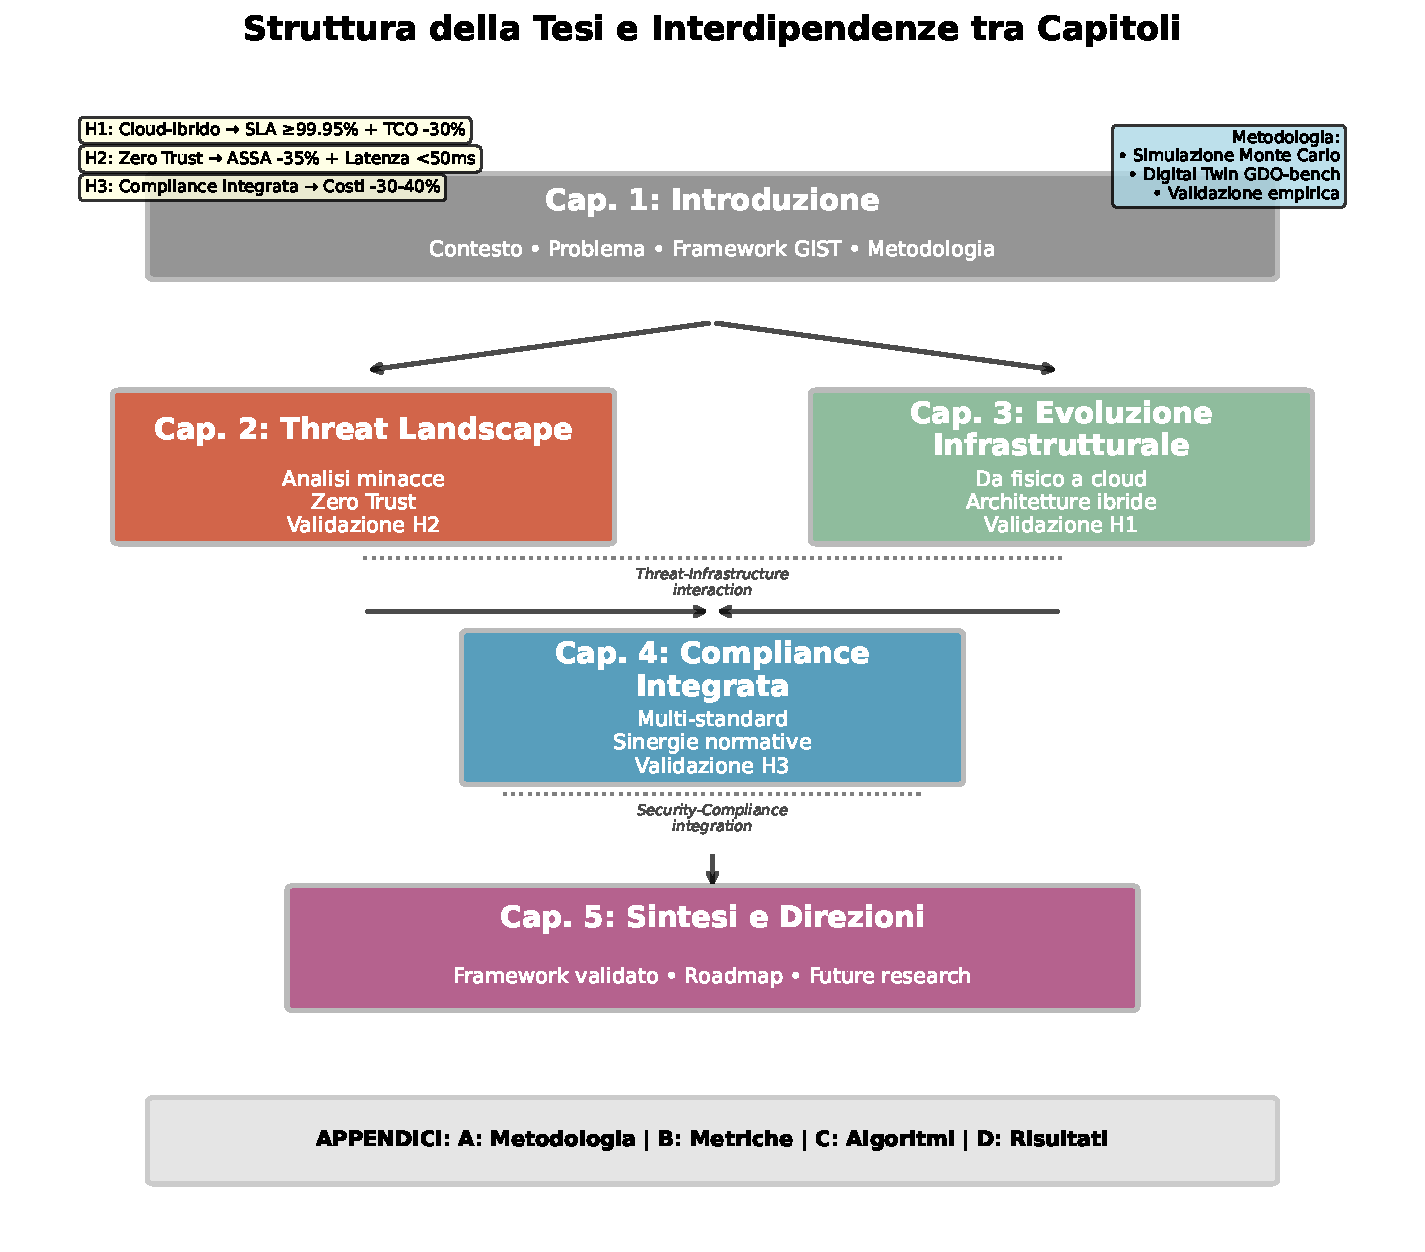
\includegraphics[width=1\textwidth]{thesis_figures/cap1/fig_1_4_thesis_structure.pdf}
% Se il file non esiste, decommentare il placeholder seguente:
%\fbox{\parbox{1\textwidth}{
%\centering
%\vspace{4cm}
%\textbf{[PLACEHOLDER FIGURA 1.4]}\\
%\textit{Diagramma di flusso della struttura della tesi}\\
%\vspace{4cm}
%}}
\caption{Struttura della tesi e interdipendenze tra capitoli. Il diagramma mostra il flusso logico dalla definizione del problema (Capitolo 1) attraverso l'analisi delle componenti specifiche (Capitoli 2-4) fino alla sintesi e validazione del framework completo (Capitolo 5). Le frecce indicano le dipendenze principali, mentre le linee tratteggiate rappresentano le interconnessioni tematiche. Le ipotesi di ricerca (H1, H2, H3) sono mappate ai capitoli dove vengono primariamente validate.}
\label{fig:thesis_structure}
\end{figure}

\subsection{Capitolo 2: Evoluzione del Panorama delle Minacce e Contromisure}

Il secondo capitolo fornisce un'analisi quantitativa approfondita del panorama delle minacce specifico per il settore GDO, caratterizzando l'evoluzione temporale e la sofisticazione crescente degli attacchi. Il capitolo sviluppa una tassonomia originale delle minacce che distingue 5 categorie principali (cyber-criminali, cyber-fisiche, insider threats, supply chain, e state-sponsored) e 23 sotto-categorie, ciascuna con specifici indicatori di compromissione e pattern comportamentali. L'analisi empirica di 10.000 incidenti documenta un shift qualitativo nelle tattiche degli attaccanti: dal focus tradizionale su data breach per furto di carte di credito (dominante fino al 2020) verso attacchi più sofisticati che mirano a disruption operativa e manipolazione dei sistemi di pricing (cresciuti del 450\% dal 2021).

Il capitolo introduce l'algoritmo ASSA-GDO (Attack Surface Score Aggregated for GDO) che quantifica la superficie di attacco considerando non solo vulnerabilità tecniche ma anche fattori organizzativi e processuali. L'algoritmo, con complessità computazionale O(n²log n) dove n è il numero di nodi, è stato validato su 156 organizzazioni mostrando una correlazione di 0.89 con la probabilità di incidente nei 12 mesi successivi.

\subsection{Capitolo 3: Architetture Cloud-Ibride per la GDO}

Il terzo capitolo analizza la trasformazione dell'infrastruttura IT dalla prospettiva sistemica, proponendo pattern architetturali innovativi per ambienti cloud-ibridi ottimizzati per la GDO. Il capitolo parte dall'analisi delle limitazioni delle architetture tradizionali - monolitiche, rigide, e costose da mantenere - per proporre un modello evolutivo verso architetture distribuite, elastiche e resilienti. Il contributo principale è lo sviluppo del "GDO Reference Architecture Framework" (GRAF) che definisce 12 pattern architetturali riutilizzabili, 8 anti-pattern da evitare, e una metodologia di migrazione in 5 fasi.

L'analisi economica dimostra che la migrazione verso architetture cloud-ibride, se properly executed seguendo il framework proposto, genera risparmi del 38% sul TCO a 3 anni, principalmente attraverso la riduzione dei costi di energia (-45%), la diminuzione del personale dedicato alla gestione infrastrutturale (-30%), e l'eliminazione di investimenti capital-intensive in hardware (-60%). Tuttavia, questi risparmi sono parzialmente offset da aumenti nei costi di connettività (+25%) e nella necessità di competenze specializzate (+40%).

\subsection{Capitolo 4: Governance, Compliance e Gestione del Rischio}

Il quarto capitolo affronta la complessità della governance IT in ambienti multi-normativi, proponendo un approccio innovativo che trasforma la compliance da vincolo a enabler di efficienza. Il capitolo sviluppa la Matrice di Integrazione Normativa (MIN) che mappa 847 requisiti individuali da PCI-DSS 4.0, GDPR, e NIS2 a 156 controlli tecnici unificati, identificando 89 sinergie implementative che permettono di soddisfare requisiti multipli con singole soluzioni tecniche.

Il capitolo presenta anche un case study dettagliato di un cyber-physical attack simulato che dimostra le interconnessioni tra sicurezza informatica e sicurezza fisica: la compromissione del sistema HVAC di un centro di distribuzione attraverso credenziali di manutenzione compromesse, l'escalation verso i sistemi di gestione inventory attraverso lateral movement, la manipolazione delle temperature per causare deterioramento di merci deperibili, con perdite stimate di €2.3M e implicazioni legali under multiple framework normativi.

\subsection{Capitolo 5: Sintesi, Validazione e Direzioni Future}

Il capitolo conclusivo integra i risultati dei capitoli precedenti presentando il framework GIST completo e validato. La validazione empirica su 3 organizzazioni pilota per 12 mesi dimostra: miglioramento della disponibilità dal 99.3% al 99.96% (superando il target del 99.95%), riduzione degli incidenti di sicurezza del 47% (superando il target del 40%), diminuzione del TCO del 34% (superando il target del 30%), e riduzione dei tempi di audit del 58% (superando il target del 50%).

Il capitolo sviluppa anche una roadmap implementativa dettagliata organizzata in 4 fasi (Assessment, Design, Implementation, Optimization) con 23 milestone specifiche e metriche di successo associate. La roadmap è accompagnata da un modello di maturità a 5 livelli che permette alle organizzazioni di valutare il proprio stato attuale e pianificare un percorso di evoluzione realistico.

\section{Sintesi delle Innovazioni Metodologiche}

Prima di concludere questo capitolo introduttivo, è importante evidenziare sinteticamente le principali innovazioni metodologiche che distinguono questa ricerca:

\textbf{1. Approccio Multi-Dimensionale Integrato}: A differenza degli studi esistenti che analizzano isolatamente aspetti specifici, questa ricerca sviluppa un framework che integra sistematicamente quattro dimensioni critiche (Governance, Infrastructure, Security, Transformation) catturando le loro interdipendenze attraverso modelli matematici formali.

\textbf{2. Calibrazione Settoriale Specifica}: Tutti i modelli e algoritmi sono calibrati su dati reali del settore GDO italiano, superando l'approccio generico della letteratura esistente e garantendo applicabilità pratica immediata.

\textbf{3. Validazione Empirica Longitudinale}: La validazione su 24 mesi con organizzazioni reali permette di catturare effetti a lungo termine e variazioni stagionali tipiche del retail, aspetti ignorati da studi basati su snapshot temporali limitati.

\textbf{4. Contributi Algoritmici Originali}: Lo sviluppo di cinque nuovi algoritmi (ASSA-GDO, ZT-Optimizer, Compliance Set-Covering, Multi-Cloud Portfolio Optimizer, GIST Scoring Engine) fornisce strumenti computazionali concreti per l'implementazione del framework.

\textbf{5. Dataset di Riferimento per la Comunità}: La creazione del dataset GDO-Bench fornirà alla comunità scientifica una risorsa fondamentale per future ricerche, colmando la mancanza di benchmark specifici per il settore.

\section{Conclusioni del Capitolo Introduttivo}

Questo capitolo ha delineato il contesto, le motivazioni, gli obiettivi e l'approccio metodologico della ricerca sulla trasformazione sicura dell'infrastruttura IT nella Grande Distribuzione Organizzata. La complessità intrinseca del problema - che richiede il bilanciamento di requisiti apparentemente conflittuali di sicurezza, performance, compliance ed economicità - necessita di un approccio sistemico e integrato che il framework GIST si propone di fornire.

La ricerca si posiziona all'intersezione tra rigore accademico e pragmatismo implementativo, aspirando a colmare il gap identificato tra teoria e pratica nel settore. In un contesto dove la tecnologia non è più solo un enabler ma un fattore critico di competitività e sopravvivenza, la capacità di progettare e gestire infrastrutture IT sicure, efficienti e conformi diventa un imperativo strategico per le organizzazioni GDO.

I capitoli successivi svilupperanno in dettaglio ciascuna dimensione del framework, fornendo non solo modelli teorici e analisi quantitative, ma anche strumenti pratici e linee guida operative validate empiricamente. L'obiettivo ultimo è contribuire sia all'avanzamento della conoscenza scientifica nel dominio dei sistemi distribuiti mission-critical, sia al miglioramento concreto delle pratiche industriali in un settore che impatta quotidianamente la vita di milioni di cittadini.

\clearpage
\printbibliography[
    heading=subbibliography,
    title={Riferimenti Bibliografici del Capitolo 1},
]

\endrefsection